\documentclass[tikz,border=8pt]{standalone}

\usepackage{amsmath}
\usepackage{bm}
\usetikzlibrary{arrows.meta, positioning, calc}

\begin{document}

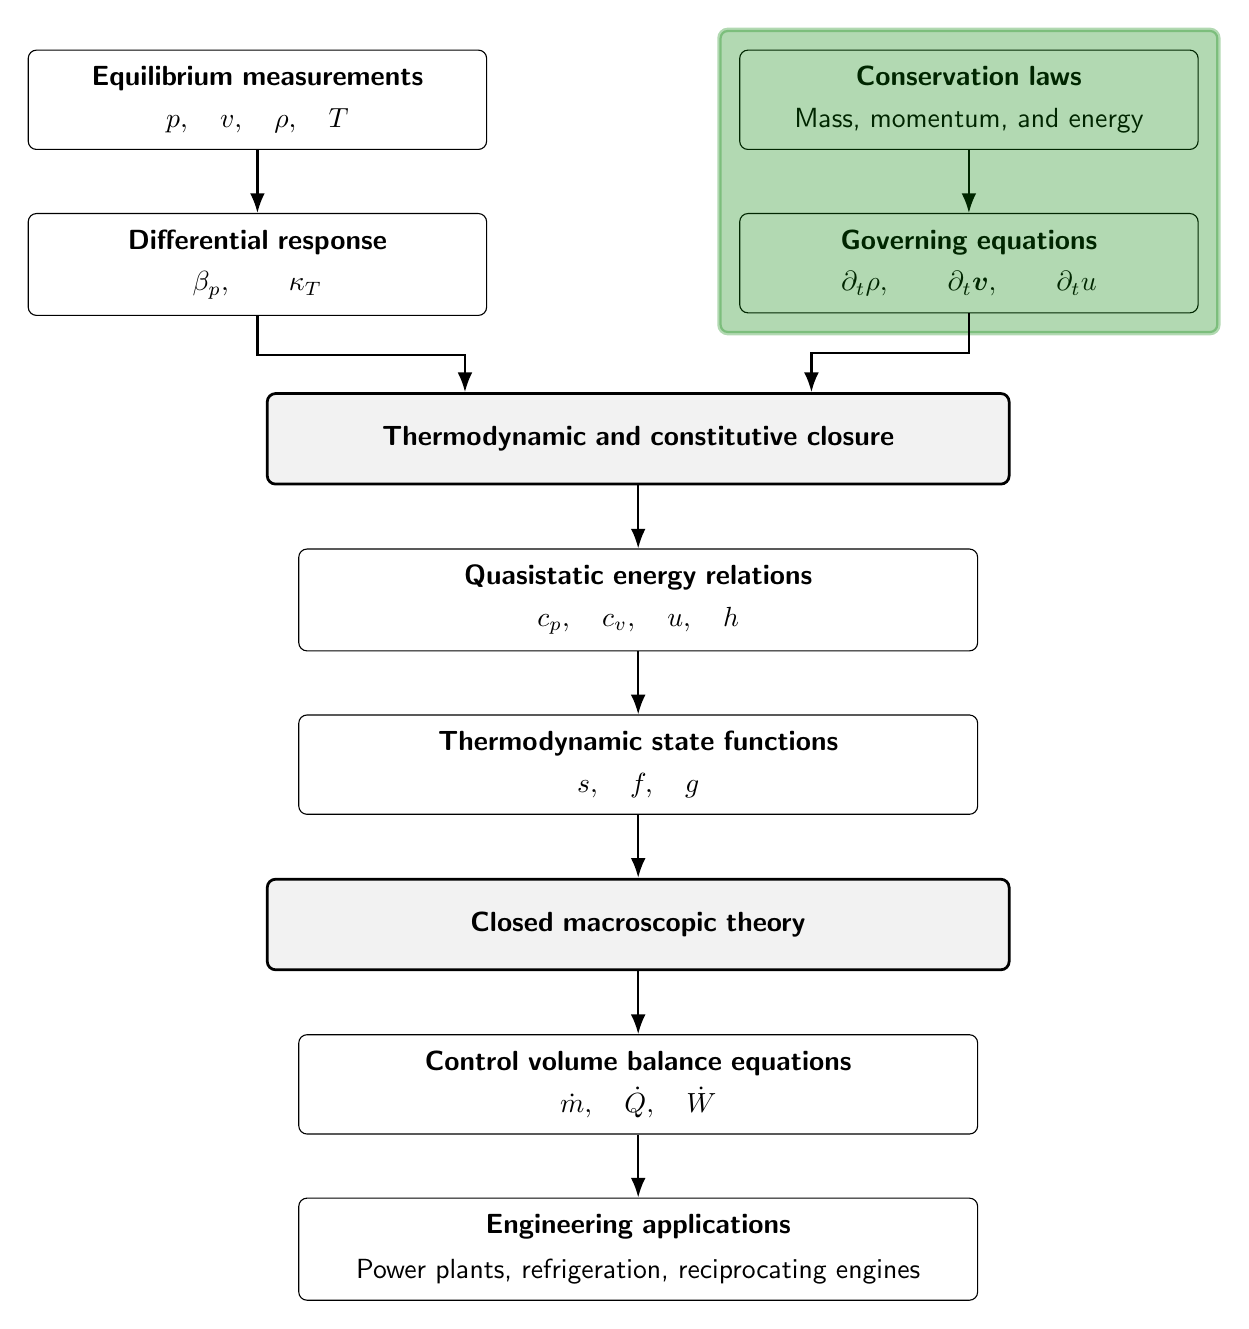
\begin{tikzpicture}[
    font=\sffamily,
    >=Latex,
    node distance=8mm and 32mm,
    flow/.style={
        -{Latex[length=2.5mm]},
        thick
    },
    flowbox/.style={
        draw,
        rounded corners=3pt,
        align=center,
        text width=5.4cm,
        minimum height=1.05cm,
        inner sep=6pt
    },
    closure/.style={
        flowbox,
        text width=9.0cm,
        minimum height=1.15cm,
        fill=gray!10,
        line width=1pt
    },
    applications/.style={
        flowbox,
        text width=9.0cm,
        minimum height=1.15cm,
        fill=gray!10,
        line width=1pt
    }
]

% -------------------------------------------------
% Thermodynamic branch
% -------------------------------------------------

\node[flowbox] (measurements) {
    \textbf{Equilibrium measurements}\\[3pt]
    $p,\quad v,\quad \rho,\quad T$
};

\node[flowbox, right=of measurements] (conservation) {
    \textbf{Conservation laws}\\[3pt]
    Mass, momentum, and energy
};

\node[flowbox, below=of measurements] (response) {
    \textbf{Differential response}\\[3pt]
    $\displaystyle
    \beta_p,
    \qquad
    \kappa_T
    $
};

\draw[flow] (measurements) -- (response);



% -------------------------------------------------
% Fluid-dynamic branch
% -------------------------------------------------

\node[flowbox, below=of conservation] (motion) {
    \textbf{Governing equations}\\[3pt]
    $\displaystyle
    \partial_t\rho,
    \qquad
    \partial_t\bm{v},
    \qquad
    \partial_t u
    $
};

\draw[flow] (conservation) -- (motion);

\fill[flowbox,ultra thick,green!50!black,opacity=0.3] ($(conservation.north east)+(0.25,0.25)$) rectangle ($(motion.south west)+(-0.25,-0.25)$);


% -------------------------------------------------
% Joining stage: closure
% -------------------------------------------------

\node[closure, below=10mm of motion, xshift=-4.2cm] (closure) {
    \textbf{Thermodynamic and constitutive closure}%\\[4pt]
};

\draw[flow] (response.south)
    -- ++(0,-5mm)
    -| ([xshift=-2.2cm]closure.north);

\draw[flow] (motion.south)
    -- ++(0,-5mm)
    -| ([xshift=2.2cm]closure.north);

    
% -------------------------------------------------
% Thermodynamic relations and state functions
% -------------------------------------------------

\node[flowbox, below=of closure, text width=8.2cm] (energy) {
    \textbf{Quasistatic energy relations}\\[3pt]
    $c_p,\quad c_v,\quad u,\quad h$
};

\node[flowbox, below=of energy, text width=8.2cm] (potentials) {
    \textbf{Thermodynamic state functions}\\[3pt]
    $s,\quad f,\quad g$
};

\draw[flow] (closure) -- (energy);
\draw[flow] (energy) -- (potentials);

% -------------------------------------------------
% Applications
% -------------------------------------------------

\node[applications, below=of potentials] (applications) {
    \textbf{Closed macroscopic theory}
};

\node[flowbox, below=of applications, text width=8.2cm] (balance) {
    \textbf{Control volume balance equations}\\[3pt]
    $\dot{m}, \quad \dot{Q}, \quad \dot{W}$
};

\node[flowbox, below=of balance, text width=8.2cm] (modeling) {
    \textbf{Engineering applications}\\[4pt]
    Power plants, refrigeration, reciprocating engines
};

\draw[flow] (potentials) -- (applications);
\draw[flow] (applications) -- (balance);
\draw[flow] (balance) -- (modeling);

\end{tikzpicture}

\end{document}
